\subsubsection{Rules for Combining Rotation-like Numbers}

\todo{rotation-like numbers = rotation tuples}
\todo{replace cycles with correct notation for cycles in full model}

\begin{figure}
    \centering
    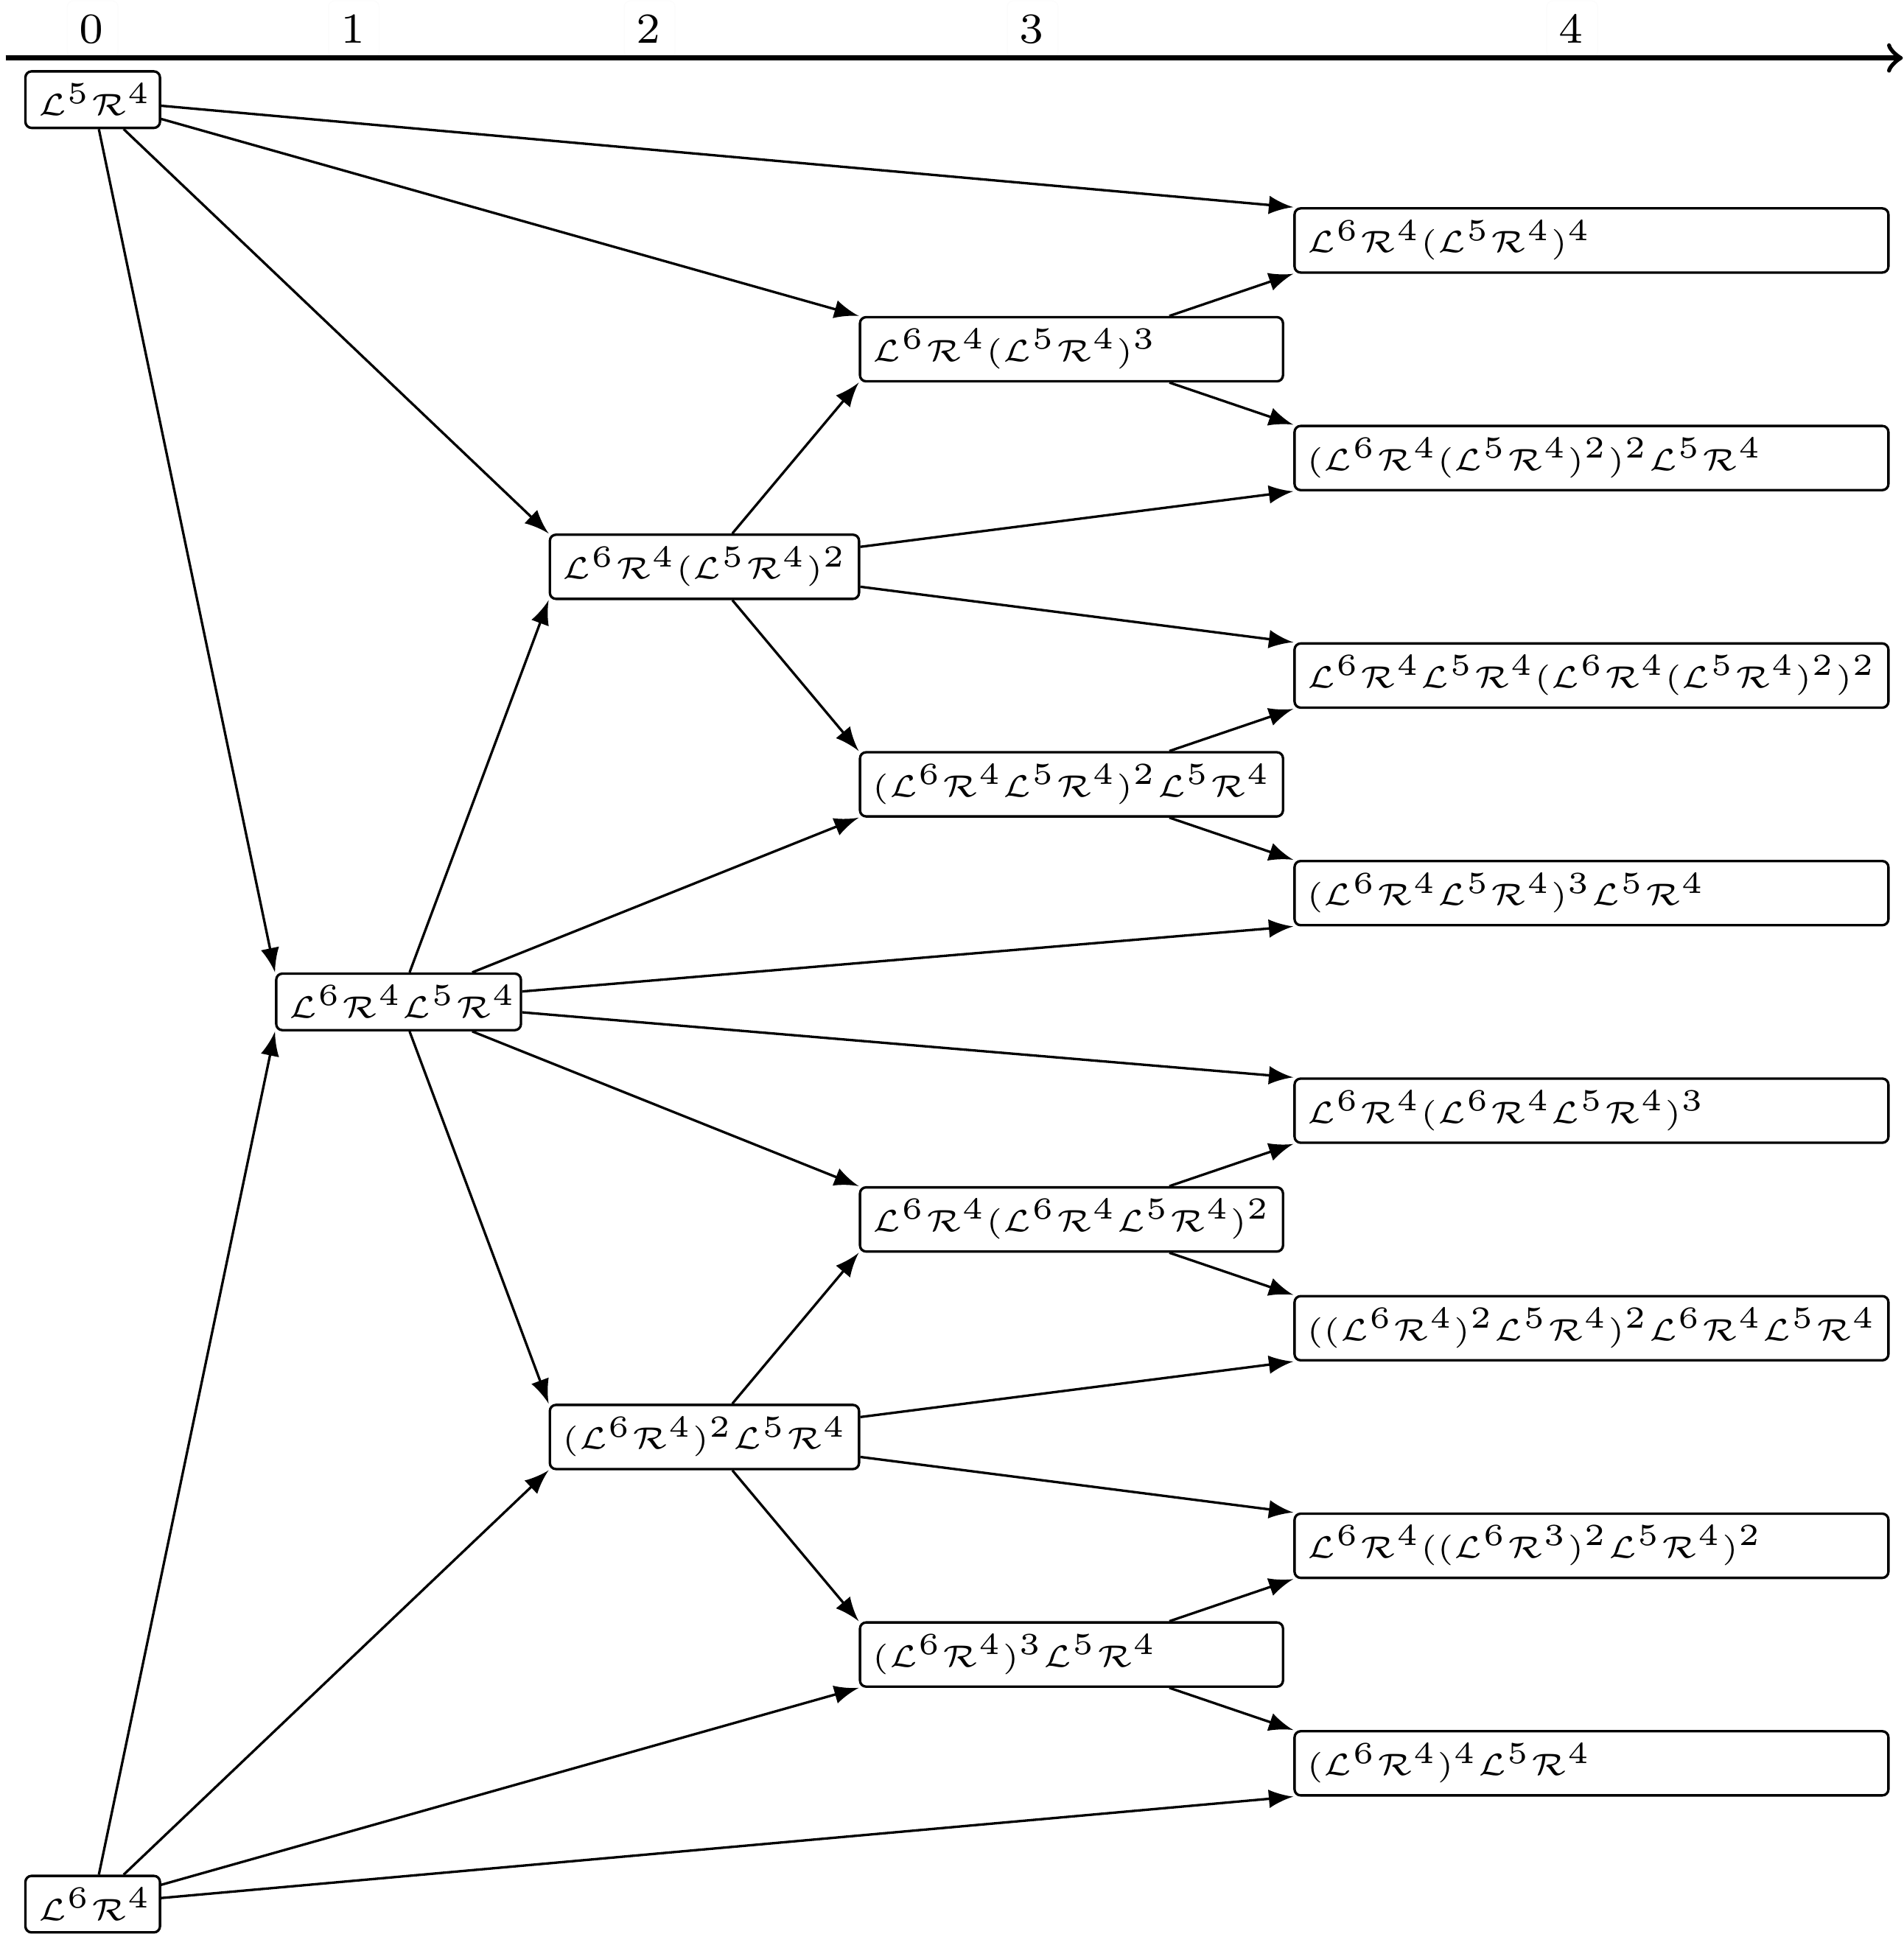
\includegraphics[width=.8 \textwidth]{FareyTrees/Minrep_Adding1_Full_RotNum/adding.png}
    \caption{Farey tree with rotation numbers}
\end{figure}

\begin{definition}[Rotation-like Numbers]
    Rotation-like numbers for symbolic sequences $\sigma$ in the full model.
    \begin{align*}
        \rho_\A(\sigma) = \dfrac{|\sigma|_\A}{|\sigma|}, \quad
        \rho_\B(\sigma) = \dfrac{|\sigma|_\B}{|\sigma|}, \quad
        \rho_\C(\sigma) = \dfrac{|\sigma|_\C}{|\sigma|}, \quad
        \rho_\D(\sigma) = \dfrac{|\sigma|_\D}{|\sigma|}
    \end{align*}
    Where $|\sigma|_\A$ is the number of symbols $\A$ in the sequence.
    Analogous for the symbols $\B$, $\C$, and $\D$.
\end{definition}

\begin{definition}[Farey Addition]
    \todo{define}
\end{definition}

\begin{theorem}
    The child node of a node with a singular cycle $\sigma$ and a node with two coexisting cycles $\varrho^a$ and $\varrho^b$ will have the following rotation-like numbers.
    We will call the cycle associated with the child node $\pi$ in the following.
    \begin{align*}
        \rho_\A(\pi) & =
        \rho_\A(\sigma) \oplus \rho_\A(\varrho^a) \oplus \rho_A(\varrho^b) \\
        \rho_\B(\pi) & =
        \rho_\B(\sigma) \oplus \rho_\B(\varrho^a) \oplus \rho_B(\varrho^b) \\
        \rho_\C(\pi) & =
        \rho_\C(\sigma) \oplus \rho_\C(\varrho^a) \oplus \rho_C(\varrho^b) \\
        \rho_\D(\pi) & =
        \rho_\D(\sigma) \oplus \rho_\D(\varrho^a) \oplus \rho_D(\varrho^b)
    \end{align*}
    \todo{volle schreibweise überall?}
\end{theorem}

\begin{proof}
    \todo{prove}
\end{proof}

\begin{theorem}
    The child node of two nodes with a singular cycle, $\sigma$ and $\varrho$ respectively, will have the following period.
    We will call the two cycles associated with the child node $\pi^a$ and $\pi^b$ in the following.
    \begin{align*}
        |\pi^a| = |\pi^b| & = \dfrac{|\sigma| + |\varrho|}{2} = |\pi|
    \end{align*}
    And its rotation-like numbers will be the following.
    \begin{align*}
        \rho_\A(\pi^a) & = \dfrac{|\sigma_1 \dots \sigma_{\frac{n+1}{2}}|_\A + |\varrho_{\frac{m+3}{2}} \dots \varrho_m|_\A}{|\pi|} \\
        \rho_\B(\pi^a) & = \dfrac{|\sigma_1 \dots \sigma_{\frac{n+1}{2}}|_\B + |\varrho_{\frac{m+3}{2}} \dots \varrho_m|_\B}{|\pi|} \\
        \rho_\C(\pi^a) & = \dfrac{|\sigma_1 \dots \sigma_{\frac{n-1}{2}}|_\C + |\varrho_{\frac{m+1}{2}} \dots \varrho_m|_\C}{|\pi|} \\
        \rho_\D(\pi^a) & = \dfrac{|\sigma_1 \dots \sigma_{\frac{n-1}{2}}|_\D + |\varrho_{\frac{m+1}{2}} \dots \varrho_m|_\D}{|\pi|} \\
        \rho_\A(\pi^b) & = \dfrac{|\varrho_1 \dots \varrho_{\frac{m+1}{2}}|_\A + |\sigma_{\frac{n+3}{2}} \dots \sigma_n|_\A}{|\pi|} \\
        \rho_\B(\pi^b) & = \dfrac{|\varrho_1 \dots \varrho_{\frac{m+1}{2}}|_\B + |\sigma_{\frac{n+3}{2}} \dots \sigma_n|_\B}{|\pi|} \\
        \rho_\C(\pi^b) & = \dfrac{|\varrho_1 \dots \varrho_{\frac{m-1}{2}}|_\C + |\sigma_{\frac{n+1}{2}} \dots \sigma_n|_\C}{|\pi|} \\
        \rho_\D(\pi^b) & = \dfrac{|\varrho_1 \dots \varrho_{\frac{m-1}{2}}|_\D + |\sigma_{\frac{n+1}{2}} \dots \sigma_n|_\D}{|\pi|}
    \end{align*}
\end{theorem}

\begin{proof} \phantom{x}
    \begin{enumerate}
        \item \todo{prove period}
        \item \todo{prove rotation-like numbers}
    \end{enumerate}
\end{proof}

\todo{last case not possible in our adding structures. proof!}

\begin{theorem}
    The child node of two nodes with two coexisting cycles, $\{\sigma^a, \sigma^b\}$ and $\{\varrho^a, \varrho^b\}$ respectively, will have the following rotation-like numbers.
    We will call the two cycles associated with the child node $\pi^a$ and $\pi^b$ in the following.
    \begin{align*}
        \rho_\A(\pi^a) & = \rho_\A(\sigma^a) \oplus \rho_\A(\varrho^a) \\
        \rho_\B(\pi^a) & = \rho_\A(\sigma^a) \oplus \rho_\A(\varrho^a) \\
        \rho_\C(\pi^a) & = \rho_\A(\sigma^a) \oplus \rho_\A(\varrho^a) \\
        \rho_\D(\pi^a) & = \rho_\A(\sigma^a) \oplus \rho_\A(\varrho^a) \\
        \rho_\A(\pi^b) & = \rho_\A(\sigma^b) \oplus \rho_\A(\varrho^b) \\
        \rho_\B(\pi^b) & = \rho_\A(\sigma^b) \oplus \rho_\A(\varrho^b) \\
        \rho_\C(\pi^b) & = \rho_\A(\sigma^b) \oplus \rho_\A(\varrho^b) \\
        \rho_\D(\pi^b) & = \rho_\A(\sigma^b) \oplus \rho_\A(\varrho^b)
    \end{align*}
\end{theorem}

\begin{proof}
    \todo{prove}
\end{proof}

In the usual case with two symbols, the rotation numbers are monotone.
In our case, this is not true when considering both rotation-like numbers of coexisting cycles.
The first step is a counter example, $\dfrac{6}{19} > \dfrac{6}{20}$ and $\dfrac{6}{19} > \dfrac{5}{18}$.
But when considering the farey sum of the rotation-like numbers of coexisting cycles, the monotony holds.

\begin{theorem}{Monotony of Rotation-like Numbers in the Full Model}
    The rotation-like numbers for one symbol are monotone in the farey tree of a period-adding structure in the full model, when considering the farey sum of the rotation-like numbers of coexisting cycles.
    \todo{sentences too long and complicated in enumeration}
    \begin{enumerate}
        \item The rotation-like numbers that correspond to the cycle of a child node of a parent node with a singular cycle and a parent node of two coexisting cycles, is in between the corresponding rotation-like number of the parent node with a singular cycle and the corresponding sum of rotation-like numbers of the parent node with two coexisting cycles.
              \begin{align*}
                       & \rho_X(\sigma) < \rho_X(\pi) < \rho_X(\varrho^a) \oplus \rho_X(\varrho^b) \\
                  \lor & \rho_X(\sigma) > \rho_X(\pi) > \rho_X(\varrho^a) \oplus \rho_X(\varrho^b)
              \end{align*}
        \item The farey sum of the rotation-like numbers that correspond to each coexisting cycle of a child node of two nodes with a singular cycle each, is in between the corresponding rotation-like numbers of the parent nodes.
              \begin{align*}
                       & \rho_X(\sigma) < \rho_X(\pi^a) \oplus \rho_X(\pi^b) < \rho_X(\varrho) \\
                  \lor & \rho_X(\sigma) > \rho_X(\pi^a) \oplus \rho_X(\pi^b) > \rho_X(\varrho)
              \end{align*}
    \end{enumerate}
\end{theorem}

\begin{proof}
    \todo{prove}
\end{proof}

\todo{rotation numbers in the sense of poincare follow monotony directly, but coexisting cycles have same rotation numbers}

rotation number of coexisting cycles = rotation number of cycle in halved model

rotation number of single cycle = 2 $\otimes$ rotation number of cycle in halved model